\onehalfspacing \chapter {Analyse du monde de l'édition vidéo
professionnel}

\minitoc \mtcskip \newpage

\doublespace

\paragraph{}

%désolé Thibault mais je ne comprends pas bien cette première phrase:

%à  quoi peut-on s'attendre exactement ? Est-ce plus claire?

Le montage vidéo professionnel est un domaine très vaste, et l'on
peut s'attendre à ce que la palette de fonctionnalités nécessaires
à la création des différents formats d'œuvres audiovisuelles
varient fortement en fonction du type de contenu. Afin d'étudier les
possibilités d'avenir des logiciels libres dans ce domaine, il nous
faut définir, pour en connaître les différents besoins:

\begin{itemize} \setlength{\itemsep}{2mm}

  \item {les cas d'utilisation (plus communément appelées use cases
    \index{use cases})} \glossary{name={Cas d'utilisation (use case)},
    description={un cas d'utilisation définit une manière d'utiliser
    le système et permet d'en décrire les exigences fonctionnelles.}}

  \item {les fonctionnalités qui en découlent}

\end{itemize}


\paragraph{}

Nous allons donc définir les principaux cas d'utilisation en fonction des
différents formats de productions audiovisuelles et ainsi en déduire les
fonctionnalités nécessaires pour y répondre.

\paragraph{}

Ensuite nous analyserons la base commune des fonctionnalités nécessaires
à la réalisation de ces différents types de production.  Pour finir
nous verrons s'il existe une diversité dans les besoins, et essayerons
de trouver les fonctionnalités qui sont propres à chaque type de
production. Cette première analyse a pour but de clarifier les besoins
des professionnels afin de déterminer par la suite ceux auxquels les
logiciels libres répondent déjà, ceux auxquels on peut prétendre
répondre dans un futur proche, et ceux qui sont hors du scope actuel
des technologies libres.

\newpage

\section{Les bases de l'édition vidéo}

\paragraph{}

Tout d'abord, il est évident que, pour qu'un logiciel de montage
puisse répondre aux besoins des professionnels, les fonctionnalités
basiques de l'édition vidéo non linéaire doivent être couvertes.
Cette partie a pour but de définir quelles sont ces fonctionnalités,
et de les expliquer succinctement:

\subsection{Définition des termes techniques}

\paragraph {}

Du fait de l'importance des termes suivant pour la compréhension de
ce document, il est nécessaire qu'ils soient définis au sein même
de celui-ci.

\paragraph{Les Footages}

Les Footages correspondent à toutes les sources brutes qui ont été
enregistrées et à partir desquelles le monteur va créer le rendu
final de l'œuvre audiovisuelle.

\paragraph{Les Clips}

Les Clips correspondent dans les faits à un Footage édité (retouche
des couleurs, modification de la durée, ajout d'effets\ldots) par le
monteur afin de l'utiliser dans le contexte précis d'une œuvre finale.

\subparagraph{Les Templates}

Dans l'édition video, on parle de Template pour définir un moule de
montage. Il permet au monteur de monter très rapidement des oeuvres en
s'assurant que le rendu entre dans un cadre défini précédemment.

\paragraph{Colorimétrie (retouche des couleurs)}

En édition vidéo la colorimétrie est l'art de retoucher les couleurs,
les étalonner au travers des différents clips.

\paragraph{Les effets vidéos}

Les effets vidéo sont des effets visuels qui permettent de modifier
l'image d'une vidéo de manière simple (à l'inverse des effets spéciaux
qui modifie la vidéo de manière plus complexe).

\begin{wrapfigure}{r}{0.5\textwidth}

   \vspace{-20pt}

    \begin{center}

      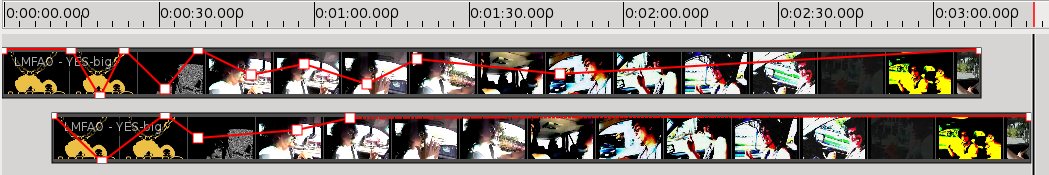
\includegraphics[width=0.48\textwidth]{images/keyframecurves}

    \end{center}

   \vspace{-30pt} \caption{Les keyframes} \vspace{-10pt} \label{Yes}

\end{wrapfigure}

\paragraph{Les keyframes}

Les keyframes définissent le début et la fin d'une animation, en
particulier dans le cadre d'effet, de texte en mouvement au dessus d'une
vidéo (dans le cadre de titres, sous-titres).

\paragraph{Speed control et time remapping}

Le speed control permet de modifier la vitesse de lecture d'un clip
dans la timeline (ralentir ou accélérer). Le time remapping est une
technique avancée de speed control, et permet de changer la vitesse de
lecture d'une partie de clip, et ainsi d' accélérer ou de ralentir des
parties d'un même clip. Cette technique est couplée aux keyframes afin
d'obtenir le résultat souhaité.

\paragraph{Gestion des Footages}

Un logiciel d'édition vidéo doit permettre d'importer les Footages
\index{Footages} à partir desquels on veut faire le montage, c'est
à dire les fichiers vidéos, audios, et images avec lesquels on
travaille. Il doit être possible de prévisualiser ces clips.

\subsection{Definition du concept d'édition timeline}

\paragraph{}

La timeline est la partie de l'interface dans laquelle on va disposer
les différents clips. Il s'agit du concept de base de l'édition vidéo
non linéaire.  Dans le cadre de l'édition timeline quelques fonctions
sont absolument indispensables, et il est nécessaire de comprendre ces
différents concepts pour comprendre la suite de ce document:

\paragraph{Découpages des clips}

\begin{wrapfigure}{r}{0.6\textwidth}

  \vspace{-20pt} \begin{center}

    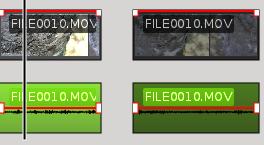
\includegraphics[width=0.38\textwidth]{images/splited}

  \end{center} \vspace{-20pt} \caption{Spliting} \label{Yes}

  \vspace{-10pt}

\end{wrapfigure}

La technique du decoupage de clip permet de diviser un Footage en
plusieurs parties afin de pouvoir les utiliser de manière indépendante.

\paragraph{}

\paragraph{Unlinking de la piste audio et de la piste vidéo}

\begin{wrapfigure}{r}{0.6\textwidth}

  \vspace{-20pt} \begin{center}

  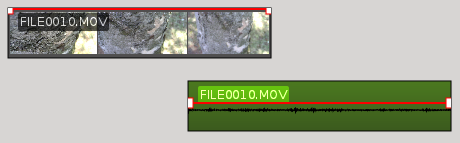
\includegraphics[width=0.38\textwidth]{images/unlinked}

  \end{center} \vspace{-30pt} \caption{Unlinking} \label{Yes}

  \vspace{-10pt}

\end{wrapfigure}

Le fait de ``de-lier'' les clips permet de gérer de manière
désynchronisée le son et la video.

\paragraph{Gestion des "in point" et  "out point" des clips}

  Permet de définir la partie d'un Footage à utiliser dans le montage
  final. Cela permet donc de redéfinir la longueur d'un clip dans la
  timeline, en ne jouant pas le début ou la fin de celui-ci.

\paragraph{}

\paragraph{Notion de layer}

\begin{wrapfigure}{r}{0.6\textwidth}

  \begin{center}

    \vspace{-20pt} 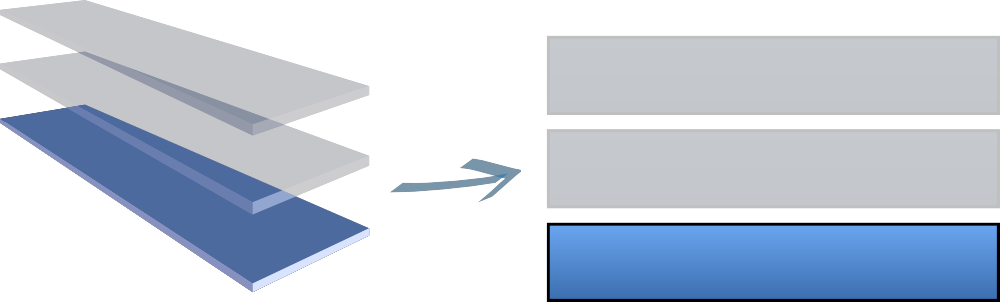
\includegraphics[width=0.38\textwidth]{images/layers}

  \end{center} \vspace{-20pt} \caption{Les layers} \label{Yes}

\end{wrapfigure}

La notion de layer est essentielle dans l'édition video avancée dans
la timeline : mixer plusieurs sources et ajouter des titres dépend de
cette fonctionnalité. Afin de comprendre, il est plus simple de faire
la comparaison avec de la peinture sur verre : on superpose plusieurs
vitres les unes au dessus des autres, chacune de ces vitres représentant
un layer. C'est la superposition des dessins de chacune des plaques
qui va nous révéler le résultat final. De plus, il existe dans les
layers une notion d'opacité , ce qui permet d'atténuer ou de révéler
intégralement les dessins des plaques inférieures.

\newpage\section{Définition du marché par segment}

\paragraph{}

Dans un premier temps, nous allons définir et analyser les différents
formats de productions audiovisuelles professionnelles. Nous avons
interviewé un certain nombre de monteurs professionnels, afin de lister
leurs besoins, (annexes 1) et en essayant de couvrir le maximum de champs
de l'édition vidéo. Nous avons pu récolter des informations provenant
de monteurs de clips vidéos, de courts métrages, de publicités,
de documentaires, de séries télévisés, et de reportages.

\paragraph{}

La littérature dans la matière (en particulier
\cite{WorldVideoNonlinearEditingMarket}) nous propose de faire une nette
distinction entre les deux segments du marché que sont:

\begin{itemize} \setlength{\itemsep}{2mm}

  \item {le monde du contenu post-produit: il s'agit de contenu dont la
    qualité de montage final est très importante. Celui-ci peut être de
    courte durée, tels que les clips vidéos ou publicités, ou bien de
    longue durée, tels que les films ou les séries télévisées. Mais
    il faut toutefois faire une différence entre ces derniers puisque
    la qualité du rendu final des films implique d'autres standards en
    terme de montage}

  \item {le monde de la production diffusée: il s'agit du contenu
    retransmis à la fois, sur internet, et sur les chaînes de
    télévisions et dont la création et la retransmission rapide
    impliquent des moyens spéciaux qui permettent de créer et
    retransmettre le contenu dans un temps restreint, voir en direct.}

\end{itemize}

\paragraph{}

Certes les deux mondes ont des contenus différents, mais surtout
ils ont des contraintes différentes, ce qui implique des divergences
importantes en terme de besoin de fonctionnalités. Nous allons donc
nous intéresser à ces deux domaines et découper notre analyse à
partir de cette distinction. Tout d'abord, nous nous intéresserons aux
fonctionnalités logicielles nécessaires à la production de contenu
post-produit. Nous analyserons ensuite les besoins intrinsèques à la
production de contenu visant le monde de la vidéo diffusée. Puis nous
essayerons de voir où se situe la frontière entre ces deux mondes afin
d'évaluer l'investissement pour les logiciels de montage vidéo libres
nécessaire pour répondre à ces marchés.

\paragraph{Le monde du contenu post-produit}

\subparagraph{}

Le monde du contenu post produit est assez vaste et au premier abord
il peut apparaître comme étant tout le contenu qui n'est pas diffusé
instantanément. Dans les faits, la distinction est plus complexe, et il
s'agit d'œuvres audiovisuelles dont le temps de post production n'est
pas un critère de première d'importance pour le choix des moyens mis
en place sur ce sujet.

\subparagraph{}

De ce fait, les formats suivants peuvent être considérés comme étant
post produits:

\paragraph{Les courts métrages}

\subparagraph{}

Les courts métrages concentrent une histoire en moins de 35 minutes. Ils
sont donc soumis à des contraintes importantes. Ils répondent à
une exigence de concision et il est donc intéressant de se poser la
question pour savoir si dans ce genre d'œuvre les monteurs utilisent
des techniques qui permettent de les rendre plus dynamiques et si des
fonctionnalités spéciales sont utilisées dans ce but.

\subparagraph{}

Dans la production de ce type d'œuvre, les interviews nous ont révélé
des fonctionnalités indispensables telles que:

\begin{itemize} \setlength{\itemsep}{2mm}

  \item{Transition (fading en priorité)}

  \item{Effets basiques (par exemple le passage en noir et blanc)}

  \item{Time remapping}

  \item{Retouche des couleurs}

  \item{Création et ajout de génériques}

\end{itemize}

\paragraph {Les publicités}

\subparagraph{}

La publicité peut s'apparenter au court métrage puisqu'il s'agit de
création courte et généralement dynamique mais dont l'objectif est
différent.  Pour atteindre cet objectif (attirer des consommateurs),
les monteurs utilisent des techniques spéciales mais les fonctionnalités
du logiciel nécessaires restent identiques à celles du court métrage.

\subparagraph{}

En revanche, la qualité du rendu est très importante: ainsi des
logiciels spécialisés sont fréquemment utilisés afin de créer le
contenu (audio, effets, images\ldots).

\paragraph {Les clips vidéos}

\subparagraph{}

Le clip vidéo est un contenu visuel qui a pour but d'illustrer une
musique. Ce type de vidéos utilise souvent beaucoup d'effets spéciaux,
et demande à priori une très grande précision au niveau de la
synchronisation entre le son et l'image. La track audio dans de telle
production sera de préférence effectuée avec un logiciel dédié à
cet effet. Pour résumer, les fonctionnalités nécessaires sont:

\begin{itemize} \setlength{\itemsep}{2mm}

  \item{Création de titres complexes (Titre en mouvement, etc\ldots)}

  \item{Ajout de titres}

  \item{Ajout d'effets}

  \item{Utilisation avancé des keyframes}

  \item{Time remapping}

\end{itemize}

\paragraph {Les films}

\subparagraph{}

La production cinématographique bénéficie de budgets beaucoup plus
élevés. Les techniques employés dans le cadre de la post production
sont plus complexes et permettent de gérer avec soin la qualité
du rendu.

\subparagraph{}

Il n'a pas été possible d'interviewer de monteur de film jusqu'à
maintenant, mais le livre ``The technique of film and video editing,
History, Theory, and Practice'' \cite{TheTechniqueOfFilmAndVideoEditing}
est un bon point de départ pour comprendre le montage cinématographique
et la très grande influence qu'il a sur les autres types de productions
audiovisuelles. On peut considérer le film comme étant une oeuvre
audiovisuelle par excellence.

\subparagraph{}

Dans le monde du cinéma, le logiciel de montage vidéo est l'un des
logiciels parmi un système connecté de logiciel de post production. Des
spécialistes de différents domaines créent les parties du film,
et le monteur a pour mission de lier tout ces éléments au travers du
logiciel de montage. Les logiciels de post production sont entre autres:

\begin{itemize} \setlength{\itemsep}{2mm}

  \item{Éditeur de son}

  \item{Création d'effet}

  \item{Retouche d'image}

  \item{Création d'animation}

  \item{\ldots}

\end{itemize}

\subparagraph{}

Les logiciels à visée professionnelle ne sont donc pas forcément
utilisables dans le monde de la création cinématographique. Il
conviendra de faire une réelle différence entre ces deux univers du
montage vidéo.

\subparagraph{}

Le logiciel de montage vidéo à proprement parler ne nécessite pas
vraiment de fonctionnalités très évoluée.  Mais la caractéristique
principal auquel doit répondre les logiciels dans ce domaine est la
possibilité d'organiser de manière efficace une très grande quantité
de footages.

Les autres logiciels de post production sont bien évidemment aussi
nécessaires afin de permettre de faire le montage de films. Ce document
n'a pas pour but de détailler ces autres logiciels.

\subparagraph{}

Une autre caractéristique de la production cinématographique, qui est
une conséquence directe de l'impératif de qualité irréprochable,
réside dans le fait que les logiciels de montage doivent permettre de
visualiser chaque image du film de manière très précise (le montage
de film se fait dans certain cas en choisissant chaque image depuis un
tableau de frames \index{frame}).


\subparagraph{}

Bien que ne demandant pas vraiment de fonctionnalités très avancées,
la création de film a des besoins assez évoluées en ce qui concerne
le logiciel de montage:

\begin{itemize} \setlength{\itemsep}{2mm}

  \item{Organisation très avancée des Footages}

  \item{Création et ajout de générique}

  \item{Passerelles avec le reste des logiciels de post production}

  \item{Preview de chaque frame dans le détail}

\end{itemize}

%TODO essayer de trouver des monteurs de films!

\newpage\paragraph {Les séries télévisées}

\paragraph{}

Le niveau de qualité des séries télévisées n'étant pas aussi élevé
que pour le montage des films, les traitements sont la plupart du temps
réalisés directement dans le logiciel de montage même. Cela implique
un nombre de fonctionnalités plus important nécessairement les fonctionnalités
suivantes:

\begin{itemize} \setlength{\itemsep}{2mm}

  \item{Création et ajout de titre}

  \item{Création et ajout de générique}

  \item{Retouche des couleurs}

\end{itemize}

\paragraph {Les documentaires}

\paragraph{}

Le documentaire est assez sobre en terme de montage. Il
réside en général dans le logiciel de montage, mais ne demande pas
de fonctionnalités spéciales. Les fonctionnalités utilisées pour
produire ce type d'œuvre sont:

\begin{itemize} \setlength{\itemsep}{2mm}

  \item{Création et ajout de titre}

  \item{Création et ajout de génériques}

  \item{Retouche des couleurs}

  \item{Utilisation des keyframes}

  \item{Transition smpte\glossary{name={smpte}, description={Society of
    Motion Picture and Television Engineers, est une association
    internationale, située aux É.-U., et composée d'ingénieurs. Elle
    développe des standards vidéos (elle en a déjà plus de 400 à
    son actif), qui sont utilisés par exemple par la télévision, ou le
    cinéma numérique (Source: http://fr.wikipedia.org/)}} \index{SMPTE}}

\end{itemize}

\newpage\paragraph{Le monde du contenu diffusé}

\paragraph{}

La plupart du contenu post produit est par la suite diffusé, la
différence que l'on fait ici entre ces deux types de production
réside dans le temps de la post production.  Dans le cas des journaux
télévisés, émission de télé, la post production est soit totalement
inexistante (dans le cas du direct), soit très courte, dans le cadre
de reportages, jeux télévisés et autres types de production visant
spécifiquement la télévision.

\paragraph {Les émissions télévisées}

\paragraph{}

Suivant leur mode de production, les émissions de télévision peuvent
être classées soit dans le contenu post-produit soit dans le contenu
diffusé. Elles sont en général diffusées très rapidement après la
création du contenu (si ce n'est en direct) et c'est la raison pour
laquelle nous les considérons comme du contenu diffusé. De plus le
fait qu'elles soient produites exclusivement pour la diffusion (aucune
commercialisation matérielle n'en est faite), cette classification
paraît naturelle.

Du fait de leur temps de production très réduit, les principales
fonctionnalités en terme de logiciel de montage sont:

\begin{itemize} \setlength{\itemsep}{2mm}

  \item{Fonctionnalité de Template qui permet d'avoir un cadre général
    de montage des présentations, en temps et ainsi faire le montage
    en direct}

  \item{Titres}

\end{itemize}

\paragraph{}

Bien évidemment, dans le cadre de la création de Templates,
les transitions ``smpte''\index{SMPTE} et les effets simples sont
généralement utilisés. Mais il n'est pas rare que les Templates à
proprement parler ne soient pas créés dans le logiciel de montage,
mais plutôt dans d'autres logiciels de création de contenu audiovisuel.

\paragraph {Évènements spéciaux (sportif, d'actualité\ldots)}

\paragraph{}

En principe ce type de production audiovisuelle n'est pas post-produit. Il
s'agit de production instantanée, et pour ce type de contenu, l'outil
de montage non linéaire doit permettre de donner une impression de
contenu post-produit alors qu'il n'en est rien. Les fonctionnalités
nécessaires sont assez similaires à celles dont on aurait besoin pour
produire des émissions de télévision.

\subparagraph{}

De plus, l'acquisition étant aussi faite en direct, il doit être possible
d'intégrer le logiciel du montage dans le système de capture d'image
et de son.

De même que pour les émissions de télévision, les Template sont
généralement produits avec des logiciels dédiés à cet effet.

\subsection{Analyse des fonctionnalités communes}

\paragraph{}

On s'aperçoit donc que de nombreuses fonctionnalités sont communes aux
différents types d'œuvres. Il convient de détailler chacune de ces
fonctionnalités afin de nous rendre compte de ce qu'elles impliquent
en terme de logiciel de montage.

\paragraph{Création et ajout de titre}

\paragraph{}

Cette fonctionnalité est utilisée dans la création de plusieurs types
de contenu:

\begin{itemize} \setlength{\itemsep}{2mm}

  \item {Séries télévisés}

  \item {Documentaires}

  \item {Clips vidéos}

\end{itemize}

\paragraph{}

Bien que cette fonctionnalité soit utilisée dans différents types de
contenu, le logiciel sera le résultat de différents paramètres. Par
exemple, dans une série télévisée le travail sur les titres sera
assez limité: on aura souvent une vidéo en arrière-plan et un titre
qui fera un fondu arrière. En revanche dans le cadre de clips vidéo,
on verra fréquemment le titre en mouvement sur le rythme de la musique
par exemple. Il est nécessaire de tout mettre en oeuvre pour répondre
à la diversité de ces besoins mais il sera plus difficile aussi bien
en terme de backend qu'en terme d'interface utilisateur de répondre
aux besoins les plus spécifiques.

\paragraph{Création et ajout de générique}

\paragraph{}

La création de générique est une fonctionnalité indispensable
à laquelle de nombreux monteurs (en particulier professionnels)
font appel. Cette fonctionnalité en terme de backend est similaire à
celle des titres puisqu'il s'agit ni plus ni moins d'ajouter du texte
au dessus d'un fond, qu'il soit animé ou non. Mais en terme d'interface
utilisateur \glossary{name={Interface Utilisateur}, description={User
Interface, il s'agit du terme  très largement employé pour définir
l'interface utilisateur, en général graphique ou GUI}} il s'agit
de deux fonctionnalités différentes puisque, par définition, le
générique est un texte qui défile dans une très grande majorité
des cas, de haut en bas.

\paragraph{}

Cette fonctionnalité est l'une des plus basiques si l'on veut
répondre aux besoins des professionnels. Elle est utilisée dans la
plupart des créations vidéo et doit être à priori standardisée et
simple à utiliser dans l'interface utilisateur afin que la mise en place
des génériques (déjà écrits) soit effectuée de manière simple et
rapide par les monteurs.

\paragraph{Gestion des Keyframes:}

\paragraph{}

Les keyframes sont utilisées dans bien des domaines, mais dans beaucoup
de cas, elles sont utilisées avec parcimonie. Elles permettent dans une
vidéo, d'animer les propriétés d'éléments ajoutés par le monteur
(effets, texte, etc\ldots). Il apparaît donc nécessaire d'avoir une
gestion minimale des keyframes, en particulier pour une gestion fine
des couleurs, mais leur utilisation est rarement vraiment avancée.

\paragraph{}

Dans la création de clips en particulier, afin de dynamiser la vidéo,
les monteurs utilisent de manière intensive les keyframes.

\subsection{Fonctionnalités spécifiques} %

Dans les faits, les fonctionnalités utilisées sont assez similaires
bien que les œuvres finales soient totalement différentes.

\paragraph{}

Quelques fonctionnalités sont apparues comme vraiment propres à la
création d'un type d'oeuvre en particulier.

\paragraph{Visualisation image par image:}

\begin{wrapfigure}{r}{0.5\textwidth}

    \begin{center}

      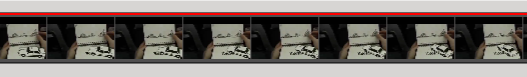
\includegraphics[width=0.48\textwidth]{images/frameByFrame}

    \end{center} \caption{Visualisation frame par frame} \label{Yes}

\end{wrapfigure}

\paragraph{}

Dans le cadre de la création de film, la prévisualisation de
chaque frame de manière précise semble être une fonctionnalité
essentielle. Cela signifie que le logiciel de montage doit permettre
de voir de manière simple chaque frame des vidéos présentes dans
la timeline. Cette fonctionnalité est aussi utile dans le cadre de la
création d'autres oeuvres, mais elle est indispensable dans le cas de
films, permettant ainsi de s'assurer de la qualité du résultat. En
effet, lors de la création d'un film, chaque frame doit être
contrôlée. Dans d'autres types d'œuvres, les exigences et les moyens
étant moins élevées, une telle fonctionnalité n'est pas indispensable.

\paragraph{Gestion avancée des Footages}

\paragraph{}

Dans le cadre de productions longues, un des problèmes auquel doit
répondre de manière satisfaisante le logiciel d'édition est la gestion
et la classification des Footages. C'est particulièrement vrai pour
les films et les séries télévisées. Dans ces types de productions
le nombre d'heures de Footages peut être très grand, et le monteur
doit dans un premier temps établir une classification des Footages. Le
logiciel de montage doit, pour répondre aux besoins des monteurs,
permettre de les ordonner de manière précise et bien pensée.

\paragraph{Intégration dans un écosystème de logiciel de post
production}

\paragraph{}

On constate, plus particulièrement dans le cadre de création de film, que le
logiciel de montage doit s'intégrer dans l'écosystème de logiciel
de post production. C'est généralement possible si ce logiciel
de montage respecte les quelques standards de la post production
d'œuvres audiovisuelles comme par exemple le Material eXchange Format
\glossary{name = {MXF}, description={Material eXchange Format ou MXF est
un conteneur utilisé par les professionnels pour les données audio et
vidéo numériques. Il s'agit d'un format défini par des standards de
la SMPTE\index{SMPTE}. (Source: wikipedia)}} \index{MXF}

\paragraph{Time remapping}

\paragraph{}

Le time remapping, comme précédemment indiqué, est particulièrement
utilisé dans la création de contenu court. Il permet d'accélérer,
où ralentir une partie d'un clip pour le rendre l'œuvre la plus
dynamique possible.

\paragraph{Gestion des Templates}

\paragraph{ }

La création de contenu non post produit demande des fonctionnalités
particulières. La fonctionnalité qui apparaît comme clé pour répondre
aux besoins liés à ce type de produit est la création de Template. Par
exemple la création de journaux télévisés ou autres évènements
sportifs demande une gestion avancée de ``moule``, ou Template, qui
permet de lier simplement les contenus des différentes caméras à un
moment donné de la retransmission.

\paragraph{ }

Cette fonctionnalité n'est pas exclusivement utilisée dans la création
de contenu en direct, mais elle est très largement utilisée dans tout
ce qui est contenu destiné à la télévision.

\paragraph{} \paragraph{}

En conclusion, on a constaté que le champ de fonctionnalité est vaste,
la plupart de ces fonctionnalités sont génériques et leur utilisation
est,par conséquent, commune à différents types d'œuvres.En revanche
ce qui varie particulièrement  est la finesse d'implémentation et le
niveau d'utilisation qu'en fait le monteur.

\newpage \section{Comparaison des principaux logiciels présents sur le
marché de l'édition vidéo professionnelle, et analyse des manques et
risques du marché}

\paragraph{}

Il conviendra d'analyser précisément les logiciels existants, qu'ils
soient propriétaires ou libres. Cette partie a pour but de rendre compte
de l'état actuel du marché des logiciels d'édition vidéo destinés
principalement aux professionnels. Cette étude portant principalement
sur les logiciels libres, ceux-ci seront évidemment inclus dans cette
analyse même si on considère que pour certains leur manque de maturité
ne leur confère pas le droit d'y figurer.

\paragraph{}

Dans cette optique, nous analyserons les points clés des logiciels.
Tout d'abord nous comparerons les fonctionnalités des logiciels, la manière
dont elles sont gérées, et nous recueillerons l'avis de professionnels
sur ces fonctionnalités et leur implémentation dans les différents
logiciels. Ensuite nous regarderons le prix de ces logiciels, nous verrons en quoi
cela peut être un argument de poids pour les logiciels libres et leur
éventuelle prise de part de marché. Nous nous concentrerons enfin
sur la documentation, livres et autres tutoriels disponibles pour ces
différents logiciels, et nous verrons quels supports sont offerts aux
professionnels pour leur utilisation.

\subsection {Historique du marché}

\paragraph{}

Les tout premiers logiciels d'édition non linéaire ont vu le jour dans
le début des années 70.  A cette époque les solutions de stockages
de données étant très limitantes, les premiers logiciels de montage
vidéo non linéaires effectivement utilisables ont vu le jour en
1989 et ceux-ci étaient basés sur les disques durs pour ce qui est du
stockage. C'est cette année là que ``Editing Machines Corp.'' et Avid
ont mis sur le marché les logiciels de montage vidéo non linéaire
ainsi que le matériel qui permettait son utilisation. Une fois de plus,
les limitations en terme de stockage de données (accès limité à
50 Gigabytes à la fois maximum), rendait l'utilisation des systèmes
de montage non linéaire inutilisables dans le domaine du cinéma,
et même dans de nombreux cas de la télévision. C'est en 1992 que
cette limitation a été surmontée: il était alors possible d'accéder
jusqu'à 7 Terabytes de données à la fois ce qui rendait envisageable
le montage de production longue de manière informatique. En
1993 Avid prend avantage de cela et s'impose comme leader mondial,
remplaçant les équipements de montage de pellicules 35mm de toutes
les principales maisons de production cinématographiques dans le
monde. Avid a été le leader incontesté du marché de l'édition
professionnel jusqu'en 2003, date à laquelle Final Cut Pro a été
considéré comme une bonne alternative à Avid par les grands acteurs
de l'édition vidéo professionnel.

\subsection{Définition des plus grands acteurs du marché}

\paragraph {Logiciels commerciaux}

\subparagraph{Avid Media Composer:}

Leader historique du marché du logiciel de montage non linéaire
professionnel. Il s'agit du produit phare de Avid Technology publié
en 1989. Depuis, ce logiciel a joué un rôle essentiel dans le
développement de ce marché.

\subparagraph{Avid Symphony:}

Evolution de Avid Media Composer, il s'agit d'une version plus complète
en terme de fonctionnalités qui a pour but de répondre aux besoins
des monteurs de productions longues tels que les documentaires et les
séries télévisées.

\subparagraph{Final Cut Pro:}

Logiciel de montage intégré dans la suite de logiciels de
post-production de Apple, Final Cut Studio. Il s'agit d'un logiciel
de montage orienté à la fois professionnel et création de film. Il
est de nos jours très utilisé et est devenu l'un des leaders mondial
du marché.

\subparagraph{Adobe Premiere Pro:}

Logiciel de montage de la suite Adobe Creative suite, il s'agit du
logiciel d'édition vidéo à visée professionnelle de Adobe System. Il
est à la fois adapté pour la création de contenu diffusé, mais aussi
de contenu post produit.

\paragraph {Logiciel en cours de libération:}

\subparagraph{Lightworks:}

Logiciel de montage actuellement commercial, très puissant, et offrant
des fonctionnalités uniques, il permet de faire parallèlement la
production diffusée et la création post-produit. Ce produit est
particulier car ses créateurs ont décidés de libérer le code source
\cite{TheLightworksOpenSourceProjectStartHere}, et ainsi  de créer une
communauté de développeurs pour en faire un projet de logiciel libre.

\paragraph {Logiciels libres:}

\subparagraph{Cinelerra:}

Logiciel de montage et de compositing libre développé principalement
par la société Héroïne \footnote{Heroine: http://heroinewarrior.com/}
et intégré par la société LMA\footnote{LMA: http://lmahd.com/}. Il
s'agit d'un logiciel de montage non linéaire avec de très nombreuses
fonctionnalités. Principalement créé pour le création de contenu
diffusé, il permet aussi de répondre aux besoins de la production
de contenu post-produit. Il s'agit du seul logiciel libre utilisé en
milieu professionnel.

\subparagraph{Kdenlive:}

Logiciel de montage libre s'intégrant dans la suite logicielle de
l'interface graphique KDE.  Ce logiciel de montage est assez complet et
peut répondre aux besoins des monteurs de contenu post-produit.

\subparagraph{PiTiVi:}

Logiciel de montage libre encore basique mais en plein développement.
Ce logiciel a pour but de répondre aux besoins du plus grand nombre,
et en particulier à ceux des professionnels de la création de contenu,
qu'il soit post produit ou non.


\subsection{Fonctionnalités}

\paragraph{}

Tout d'abord, il convient de voir quelles fonctionnalités existent
chez les différents acteurs du marché. Afin de faciliter la lecture
et avoir une vision globale de ce qui existe nous avons dessiné une
représentation sur un diagramme en toile d'araignée.  D'après les
interviews et l'analyse précédemment faite, les axes suivants ont
été choisis:

\begin{itemize} \setlength{\itemsep}{2mm}

  \item{Gestion des formats de fichiers}

  \item{Intégration dans un écosystème de post production}

  \item{Gestion des Templates}

  \item{Gestion des Footages}

  \item{Colorimétries}

  \item{Effets}

  \item{Transitions}

  \item{Support multi-platform}

\end {itemize}

\paragraph{}

Dans le schéma suivant le niveau et la qualité d'implémentation a été
prise en compte. Les retours utilisateurs ont aussi une place importante
dans cette évaluation. La plupart de ces évaluations portent sur des
données non quantifiables et c'est pour cette raison qu'aucune échelle précise
n'est donnée. Par exemple, l'ergonomie ne peut être quantifiée,
seul le ressenti des utilisateurs peut être analysé, et c'est ce
travail qui a été effectué.

\begin{figure} [H]

  \begin{center}

    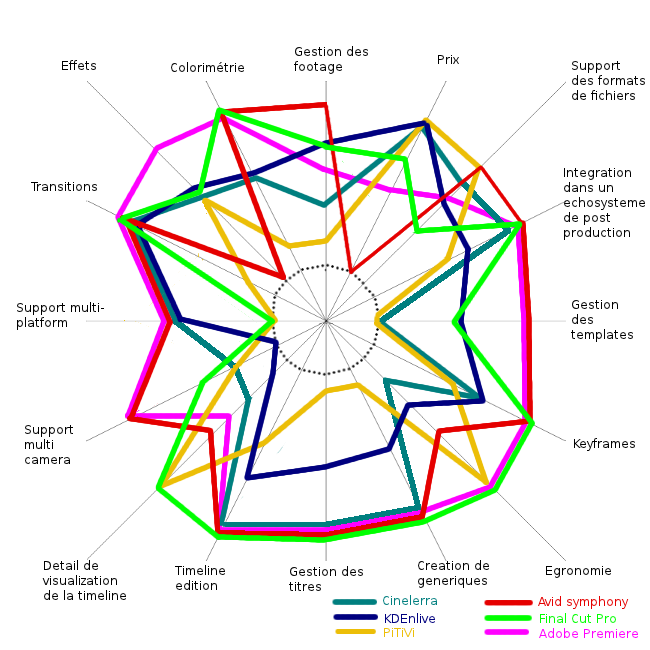
\includegraphics[width=0.9\textwidth]{images/spiderDiagramFeaturesComparision}

  \end{center}

  \caption{Comparaison des fonctionnalités des logiciels leaders sur
  le marché}

  \label{Yes}

\end{figure}

\paragraph {}

Ce schéma nous permet d'expliquer très facilement que seul le logiciel
libre Cinelerra est une place sur le marché, les lacunes de PiTiVi et
Kdenlive en terme de fonctionnalité rend leur utilisation impossible
en milieu professionnel.

\newpage

\section{Visions du marché par les professionnels du montage}

\paragraph{L'importance de la position du logiciel sur le marché}

\subparagraph{}

En ce qui concerne le choix du logiciel de montage dans une entreprise,
la connaissance que les monteurs ont du logiciel qu'ils utilisent est
essentiel.  C'est pour cela que dans de nombreux cas le premier facteur
de choix est la position de ce logiciel sur le marché de l'édition
vidéo. En effet, les différentes industries veulent avoir l'assurance qu'il
est possible de trouver de la main d'oeuvre compétente sur le logiciel
qu'elles utilisent. Mais ce n'est pas seulement la disponibilité de
personnes compétentes qui est importante, s'est également
que ces dernières puissent se former et qu'elles aient accès facilement
aux informations concernant les nouvelles résolutions des problèmes
posés par un logiciel au travers des différentes versions.

\subparagraph{}

Comme l'a souligné M. Faure lors de son interview (annexe 3), dans
son cas, il ne serait pas envisageable de changer de logiciel à moins
que le marché n'évolue. C'est à dire que l'un des critères de choix
dans son cas est la position de tel logiciel sur le marché. C'est
principalement une question de crédibilité, et donc pour éviter la
prise de risque, les professionnels préfèrent prendre la référence
du marché.

\subparagraph{}

Mais cela est principalement vrai dans les structures de taille moyenne.
Dans le cadre de petits structures, comme l'a souligné M. Veri (annexe
1) durant son interview, il serait plus logique, dans un souci de se
différencier de ses concurrents, de choisir un logiciel différent
de celui de référence. Bien évidemment ce logiciel devra répondre
convenablement à leurs besoins et permettre de satisfaire les demandes de
leurs clients. Dans son cas, M. Veri estime qu'un tel logiciel n'existe
pas et que la référence du marché (Final Cut Pro) est en réalité
la meilleure option.

\paragraph{Dépendance vis-à-vis du créateur}

\subparagraph{}

Un souci important des professionnels du montage qui ressort
des interviews est le changement de l'expérience utilisateur:
l'arrivée d'une nouvelle version est redoutée car elle demande un
temps d'adaptation pour la maitriser.  Ceci peut être illustré par
la dernière version de Final Cut Pro, qui a été très critiquée
\cite{FinalCutProXReviews}: Apple a décidé de changer le workflow
\index{workflow} des professionnels de l'édition vidéo dans la dernière
version de leur logiciel phare de ce secteur, et cela a été très mal
perçu par les professionnels. Toutefois pour M. Faure, ce problème n'est
pas trop grave, puisqu'il considère que, dans le cas où la transition
à cette nouvelle version s'avère compliquée (trop coûteuse, formation
du personnel trop onéreuse, perte de temps pour le maitriser), ils ont
toujours l'option de conserver la version courante.
Mais c'est valable seulement sur le court terme, puisqu'il n'est pas
envisageable, pour des raisons de sécurité et de support, d'utiliser
de manière commerciale un logiciel non maintenu et non supporté par
l'entreprise éditrice. Pour M. Veri en revanche, cela pose aussi un
problème important, et ayant lui même utilisé cette nouvelle version,
il considère qu'il serait préférable pour son entreprise de trouver
une autre solution.

\subparagraph{}

Dans le cadre de structures importantes, la dépendance vis-à-vis
des éditeurs est parfois considérée potentiellement dangereuse,
et donc à éviter . Par exemple, Dreamworks Picture, a décidé de
créer et de maintenir leur propre suite logiciel \cite {Dreamworks}
de post production. Leur principal objectif  est d'avoir la garantie que
leurs logiciels répondent bien à leurs besoins précis en maitrisant
leur évolution. Ils ne dépendent plus d' un éditeur externe et pour
conforter cette indépendance, cette entreprise a décidé d'utiliser
Linux comme système d'exploitation (distribution Red Hat), ce qui lui
garantit un grande liberté. De plus, la partie ``Dreamworks animations''
est cliente de la société LMA, ce qui signifie que très probablement
celle-ci utilise Cinelerra dans leur processus de post-production. De
même les sociétés de télévision française TF1 et Canal+ sont
clientes de cette même entreprise, ce qui montre bien que Cinelerra
est utilisé dans un cadre professionnel. A noter que selon M. Faure,
TF1 semble abandonner petit à petit Cinelerra au profit de Final Cut Pro.

\newpage

\section {Bilan}

\paragraph { }

Nous constatons donc que dans un marché vaste et diversifié seuls
quelques logiciels permettent à l'heure actuelle de répondre aux
besoins de la grande majorité des utilisateurs.

\paragraph{}

Les professionnels sont plutôt satisfaits des logiciels commerciaux
existants dont ils disposent avec cependant certaines limites dûs
principalement au fait que ces logiciels sont fermés et édités par une
seule entreprise (externe) . Les fonctionnalités de ces logiciels visent
à répondre à la majorité des besoins du marché, mais ils ont des
difficultés pour s'adapter à des besoins spécifiques d'entreprises .

\paragraph{}

Partant de ce constat on peut se demander si l'utilisation de logiciels
ouverts et édités par de nombreuses entreprises ne pourraient pas
prendre une place plus importante sur le marché, en offrant de nouvelles
perspectives aux acteurs du marché du montage vidéo. Les éléments
suivants peuvent être considérés comme des éléments importants sur un
marché fermé, et contrôlé par un nombre très restreint d'entreprises:

\paragraph{Plus grande autonomie vis-à-vis de la société éditrice
(développeur/designer):}

  \subparagraph{ }

    Grâce à l'utilisation de logiciel libre, il est possible de garantir
    et maintenir le logiciel en interne tout en profitant du fait que des
    personnes externes à l'entreprise, d'une part le développent, et
    d'autre part, le connaissent. Cela a pour conséquence de réduire les
    coûts d'une manière très importante tout en gardant un contrôle
    certain sur le développement du logiciel. C'est très certainement
    pour ces raisons que Dreamworks, TF1 et bien d'autres se sont mis
    à utiliser des logiciels libres.

\paragraph{Possibilité de collaboration et de communication avec les
développeurs:}

  \subparagraph{}

  Le développement des logiciels libres étant en principe fait
  publiquement, les utilisateurs (entreprises qui font le montage
  vidéos) peuvent voir l'évolution du logiciel au fur et à mesure
  de sa progression. Cela leur permet aussi de donner leur avis sur les
  directions à prendre.

\paragraph{Réduction de coût:}

\subparagraph{}

Comme l'ont souligné  M. Veri et M. Hachemi au cours de leur interview,
dans le cadre de petites structures la réduction des coûts est un
souci important.  En effet, les frais liés à l'achat de licences pour
les logiciels de montage constituent une charge financière élevée
compte tenu des prix de ces licences. L'utilisation de logiciel libre
permettrait donc, dans la très grande majorité des cas, de réduire
d'une façon significative les coûts de montage, puisque le code source
est libre d'accès.

\paragraph{Possibilité d'adaptation aux besoins précis de l'entreprise:}

\subparagraph{}

L'ouverture du code et sa mise à disposition à tous ouvre la
possibilité d'effectuer des adaptations dans le core même du logiciel
et ainsi de développer des versions spécialement adaptées aux besoins
de l'entreprise utilisatrice.

\subparagraph{}

Dans le cadre de projets commerciaux,le développement et l'adaptation de
différentes versions ne sont faites que par l'entreprise éditrice. On
peut cependant, même dans ce cadre-là, modifier, ajouter des
fonctionnalités grâce aux systèmes d'extension logicielle, mais
la flexibilité offerte par ce système reste limitée à ce que la
société éditrice veut bien mettre à disposition des développeurs
externes. (En terme d'API) \index{API} \glossary{name={API}, description={
Une interface de programmation (Application Programming Interface
ou API) est une interface fournie par un programme informatique. Elle
permet l'interaction des programmes les uns avec les autres, de manière
analogue à une interface homme-machine, qui rend possible l'interaction
entre un homme et une machine}}.

\paragraph{}

On voit que des logiciels libres sont utilisés en milieu professionnel,
mais cela reste marginal. Les opportunités que ces logiciels peuvent
apporter au monde professionnel de la post-production étant importantes,
nous allons voir comment utiliser le potentiel de ces logiciels dans
ce domaine.
